
\begin{figure}[h]
	\hspace{-3cm}
	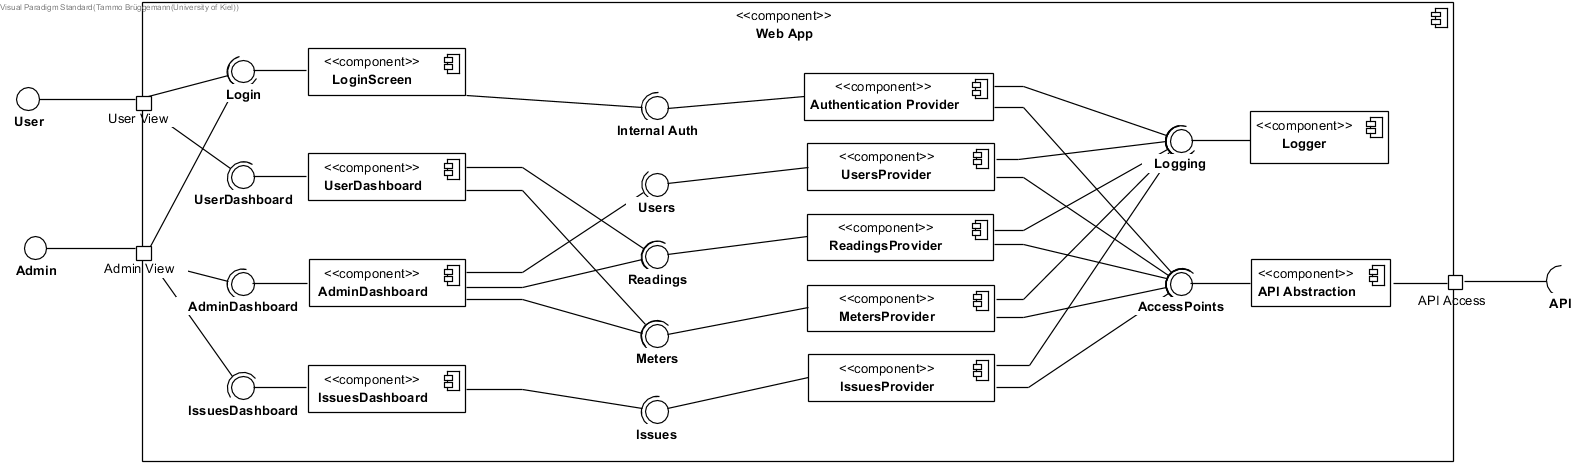
\includegraphics[scale = 0.6]{./img/Diagrams/Website-Components} 	
	\caption{Komponentendiagramm - Website} 

In der Architektur der Web-Application kann man grob in 3 Spalten unterteilen. 
\\ \\
Wobei die rechte Spalte die Service Ebene darstellt, hier befindet sich eine API Abstraction. Die API Abstraction abstrahiert alle REST-Endpunkte welche wir in der Web-Applikation benötigen. Außerdem liegt hier ein Logger, welcher uns im Entwicklungsprozess Fehlermeldungen und Logpunkte auf der Console ausgibt. Optional könnte man diese auch an ein Logservice(z.B.: Sentry) schicken.
\\ \\
In der mittleren Spalte befinden sich alle Provider. Diese stellen der Benutzeroberfläche globale Informationen (state) zur Verfügung. Hier werden API Anfragen (vom Service abstrahiert) getriggert und die entsprechenden Daten gesammelt und gecached.
\\ \\
In der linken Spalte liegen die Benutzeroberflächen, worauf die Benutzer und Administratoren zugreifen. Diese benutzen die Provider um Informationen von der API zu erhalten. 



\end{figure}
